\documentclass{report}
\usepackage{graphicx, algorithmic, algorithm2e, psfrag, amssymb, amsthm, lineno, amsfonts, amsmath, pstricks-add, bm, float, comment, amsthm, color, hyperref}
\usepackage[caption=false]{subfig}
\usepackage{booktabs, multicol, multirow} 
\hypersetup{colorlinks,breaklinks,
           linkcolor=blue,urlcolor=blue,
           anchorcolor=blue,citecolor=blue}
\newtheorem{thm}{Theorem}[section]
\newtheorem{lem}{Lemma}[section]
\newtheorem{cor}{Corollary}
\newtheorem{definition}{Definition}[section]
\newtheorem{remark}{Remark}[section]
\graphicspath{{fig/}}
\renewcommand{\figurename}{Figure }
\begin{document}
\begin{center}
\bf{Jerrad Hampton, October, 2020: Bi-fidelity PCE}
\end{center}
This is a casually written document to present a useful estimate with respect to the bi-fidelity PCE method. I am also presenting the work as I see it, to explain that estimate, which may be incorrect, or may be helpful. Traditionally, PCE would be an estimate that did not have a spatial component, only a stochastic component. As such the approximation looks like
\begin{align}
\label{eq:pce_old}
\hat{u}(\bm{\xi}) = \mathop{\sum}\limits_{k=1}^{P}c_k\psi_k(\bm{\xi}), 
\end{align}
where $\xi$ is of some stochastic dimension $d$, and $\{\psi_k\}$ are orthogonal polynomials with respect to the distribution of the $d$-dimensional random vector $\bm{\Xi}$, and $P$ is identified as a subset of those orthogonal polynomials of lower order, up to e.g. a total-order of $p$.

The key difference that allows the bi-fidelity PCE to function well, is that the problem now has spatial components, which we will denote by a vector $\bm{x}$. Now we have a representation of the approximation given by
\begin{align}
\label{eq:pce_new}
\hat{u}(\bm{x},\bm{\xi}) = \mathop{\sum}\limits_{k=1}^{P}c_k\psi_k(\bm{x},\bm{\xi}).
\end{align}

We need basis functions, $\psi_k(\bm{x},\bm{\xi})$, which are orthogonal with respect to a measure related to both the spatial and stochastic domains, but also useful for approximating the function. Fortunately, this problem has already been solved for forward UQ simulation with random spatial functions known as KLE. However, there are different correlation functions, and one or more correlation length parameters. That is, the space of potential KLE functions is large. 

In what I received, this identification of the KLE was not clearly explained, and these details may matter. In the examples, it seems that this identification is concerned with reducing a stochastic dimension from $P$ to $r$, where the spatial variance is absorbed into the coefficients, and that is the approach I take here. Specifically we want to change (\ref{eq:pce_new}) to
\begin{align}
\label{eq:pce_compressed}
\hat{u}^{(r)}(\bm{x},\bm{\xi}) = \mathop{\sum}\limits_{k=1}^{r}c_k(\bm{x})\eta_k(\bm{\xi}),
\end{align}
for some new functions $\eta_k$. This is a rank-reduction compression we are able to address, with the bi-fidelity approximation error. Let $\bm{\Psi}_{N,P}$ denote the matrix with $\bm{\Psi}(i,j) = \psi_j(\bm{x},\bm{\xi}_i)$, let $\bm{c}_{P,1}$ denote a vector of coefficients, and let $\bm{u}_{N,1}(i) = u(\bm{x},\bm{\xi}_i)$, the evaluation of the solution for the $i$th realized random variable. The method employed in what I received is to instead have $\bm{C}_{P,M}$, and $\bm{U}_{N,M}$ where $M$ is the number of spatial points sampled, giving (with transposes to this problem in what I was sent, which I'll ignore here)
\begin{align}
\label{eq:mat_original}
\bm{\Psi}\bm{C}_{P,M} = \bm{U}.
\end{align}
 In this form, the functions $\psi_k$ above have been separated into a stochastic function, which resides in $\bm{\Psi}$, and a spatial function, which is absorbed into $\bm{C}$.\\
 
We perform the bi-fidelity method to approximate $\bm{U}$. The theorem we already have bounds,
\begin{align}
\label{eq:U_bound}
\|\bm{U}_H - \bar{\bm{U}}_H\|_F,
\end{align}
for $\bar{\bm{U}}_H$ constructed through the different bi-fidelity algorithm that does not update the coefficient matrix $\bm{C}$. We use $\hat{\bm{U}}$ for this version's construction, which does update the coefficient matrix. The method works best if the spatial information is highly compressible, and if it is not (\ref{eq:U_bound}) will be large, with or without the coefficient update. However, the recomputation of the coefficient matrix $\bm{C}$ makes this method more adaptive, but also makes that bound from the non-updating algorithm generally looser, and more difficult to apply.\\

Connected to the bi-fidelity method, we have to identify the $r$ new basis functions $\eta_i$, and the matrix,
\begin{align}
\label{eq:eta_def}
\bm{\eta}_{N,r} := \bm{\Psi}_{N,P}\bm{P}_{P,r}(\bm{U}^{(r)}),
\end{align}
have the name motivated by $\eta$ in what I was sent. Specifically, $\eta_i$ represents the function
\begin{align}
\label{eq:eta_function_def}
\eta_{i}(\bm{\xi}) = \mathop{\sum}\limits_{k=1}^P\bm{\beta}(i,k)\psi_{k}(\bm{\xi}),
\end{align}
where the affect of the associated projection is given in the coefficients of the orthogonal matrix, $\bm{\beta}$. These $\eta_i$ are thus orthogonal, and this orthogonality is critical to the $\ell_2$-approximation theory.\\

This gives the matrix equation which will be used for the final approximation for the PCE itself,
\begin{align}
\label{eq:mat_final}
\bm{\eta}_{N_H,r}\bm{C}_{r,M_H} = \bm{U}^{H}_{N_H,M_H}(\bm{\eta}).
\end{align}
That is, $\{u_i\}_{i=1}^{M_H}$ are approximated by $\{\eta_i\}_{i=1}^r$, by a set of $r$ coefficients for each of the $M_H$ points. Here, as in what I received, I perform this approximation by $M_H$ independent least squares regressions, which is equivalent to doing the Frobenius regression on the entire matrix. This is the key approximation with high-fidelity samples.\\

The key low-fidelity computation is the basis identification, specifically how well can the high-fidelity problem be reconstructed by $r$ spatially varying functions. In what I was sent, this has a claimed connection to a KLE, and there are similarities, but this approach does not progress through identifying a covariance kernel, and eigenvalues/functions of it. However, being a KLE or not does not matter for the approximation here.\\

To this end, I state our previous bi-fidelity theorem with the matrices that we need. Here we use $\bm{U}^T_H := \bm{U}_{N,M_H}$ for $\bm{H}$, and $\bm{U}^T_L :=\bm{U}_{N,M_L} $ for $\bm{L}$, and using a hat to denote the rank $r$ bi-fidelity or low-fidelity reconstruction, respectively, of the matrix. Both of these use only the realizations of the model, and neither of these involve computing PCE coefficients. The transposes are to avoid making changes to the theorem, and do not effect the outcome as the $\|A\|_2 = \|A^T\|_2$. I've also changed $\rho_k(\tau)$ as as to avoid needing to put minimums in the later estimates.

\begin{thm}
\label{thm:bifi}
For any $\tau\ge 0$, let 
\begin{align}
\epsilon(\tau) = \|\bm{U}_H^T\bm{U}_H - \tau \bm{U}_L^T\bm{U}_L\|_2.
\end{align}
Let $\bar{\bm{U}}_H$ and $\bar{\bm{U}}_L$ be corresponding static coefficient bi-fidelity estimates of rank $r$ with coefficients $\bm{C}_L$, and let $\sigma_k$ denote the $k$th largest singular value of $\bm{U}_L$. Then,
\begin{align}
 \|\bm{U}_H - \bar{\bm{U}}_H\|_2 &\le \rho_k(\tau);
\end{align}
 where $\rho_k(\tau)$ is defined by
 \begin{align}
 \rho_k(\tau) &:= \mathop{\min}\limits_{\tau,k\le\mbox{rank}(\bm{U}_L)} (1+\|\bm{C}_L\|)\sqrt{\tau\sigma_{k+1}^2 + \epsilon(\tau)} + \|\bm{U}_L-\bar{\bm{U}}_L\|\sqrt{\tau + \epsilon(\tau)\sigma_k^{-2}}.
\end{align}
When $k = rank(\bm{A}_L)$, we set $\sigma_{k+1}=0$.
\end{thm}
\begin{remark}
 I note again that this theorem does not easily apply to this algorithm, as the coefficient matrix $\bm{C}_L$ is not reused for this bound. However, this bound can still provide an estimate of truncation error. This estimate relies on the Gramian estimate, which relies on high-fidelity samples, and it may be more efficient to simply perform the a posteriori error analysis with the new $\bm{C}$.
\end{remark}

We also have the theorem from our $\ell_2$ paper, that I find more easily applied, though other versions can be used. First, let's define the coherence. As we aren't using importance sampling, this can be simplified by removing the weight function. For presentation, I will ignore the more complicated coherence, and in the paper that complicated coherence has a the probability for $\mathcal{E}$ having an extra $1/r$ term which could be quite large. Let the coherence be defined as
\begin{align}
\label{eq:coherence_def}
 \mu_2 := \mathop{\sup}\limits_{\bm{\xi}\in\Omega}\mathop{\sum}\limits_{k=1}^{r}|\eta_k(\bm{\xi})|^2.
\end{align}
We note that under coherence optimal conditions, $\mu_2=r$, and such conditions can be guaranteed by importance sampling. Additionally, define the truncation error $\delta_i(\bm{\xi})$ to be the function achieving the minimum $L_2$ distance between $u_i(\bm{\xi})$ and the space of approximations from linear combinations of the basis functions $\{\eta_k(\bm{\xi})\}_{k=1}^{r}$. That is $\delta$ is the $\epsilon$ of the $\ell_2$ paper, which has been changed as it may be confused with the $\epsilon(\tau)$ used in the bi-fidelity estimate. We now present Theorem 2.1 of the $\ell_2$ paper. We note that the error $\nu_i$ in this theorem is the useful bound that we seek.
\begin{thm}
\label{thm:ez_pce}
Let
\begin{align}
\hat{u}_i(\bm{\Xi}) = \mathop{\sum}\limits_{k=1}^r \hat{c}(i,k)\eta_k(\bm{\xi}),
\end{align}
where $\hat{c}_i$ is the least-squares solution. It follows that for $\mathcal{E}$, which is independent of $i$, and is a sampling event that occurs with probability
\begin{align}
\label{eqn:rare_prob}
\mathbb{P}(\mathcal{E}) \ge 1-2r\mbox{exp}(-0.1N_H\mu_2^{-1}),
\end{align}
that
\begin{align}
\label{eq:small_nu_bd}
 \nu_i := \mathbb{E}\left(\|u_i(\bm{\Xi})-\hat{u}_i(\bm{\Xi})\|^2_{L_2(\Omega,f)};\mathcal{E}\right) \le \left(1+\frac{4\mu_2}{N_H}\right)\mathbb{E}(\delta^2_i(\bm{\Xi})),
\end{align}
where $\mu_2$ is as in (\ref{eq:coherence_def}), and
\begin{align}
 \mathbb{E}\left(X;\mathcal{E}\right) = \int_{\mathcal{E}}X(\bm{\xi})f(\bm{\xi})d\bm{\xi} = \mathbb{E}(X|\mathcal{E})\mathbb{P}(\mathcal{E})
\end{align}
denotes the expectation restricted to the event (also known as restricted expectation), and is closely related to conditional expectation.
\end{thm}
\begin{remark}
 I note here that this error bound is for each point in space. The error from the bi-fidelity approximation can be concentrated in certain spatial regions, and this is likely to apply to the PCE approximations for these $M_H$ points as well. The error from each point can be accumulated, as we do in the final corollary here.
\end{remark}

Now we have the new, original, theorem that ties these approximations together.
\begin{thm}
\label{thm:new_pc}
For $\mathcal{E}$  as in Theorem~\ref{thm:ez_pce}, and from that theorem, it follows that,
\begin{align}
\label{eq:large_nu_bd}
 \nu_i& := \mathbb{E}\left(\|u_i(\bm{\Xi})-\hat{u}_i(\bm{\Xi})\|^2_{L_2(\Omega,f)};\mathcal{E}\right)\\
 \label{eq:large_nu_bd2}
      &\le \left(1+\frac{4\mu_2}{N_H}\right)\left(\frac{\Theta_{N_H}}{N_H}\|\bm{U}_H(:,i)-\hat{\bm{U}}_H(:,i)\|^2_2\right),
\end{align}
Here $\bm{U}_H$ is the $N_H\times M_H$ matrix of high-fidelity data; $\bm{C}_L$ is the coefficient matrix associated with $\hat{\bm{U}}_H$, which is the bi-fidelity approximation to $\bm{U}_H$; and $\Theta_{N_H}$ is a random variable that converges almost surely to $1$ as $N_H\rightarrow\infty$.
\end{thm}
\begin{remark}
 We note that $\nu_i$ does not tend to zero as $N_H\rightarrow \infty$. The first term tends to $1$, as $\mu_2$ is finite and does not vary with $N_H$. However, the second term's $\|\bm{U}_H(:,i) - \hat{\bm{U}}_H(:,i)\|^2_2$, grows with $N_H$, such that the second term converges to a constant, a mean squared error in approximation from using the $r$ basis functions to approximate $\bm{U}_H$, derived from $\mathbb{E}(\delta^2_i(\bm{\Xi}))$.\\
 
 We also note that $\Theta_{N_H}$ depends on the realizations of the random variables $u(\bm{\Xi})$, and the bi-fidelity reconstruction which fill the vector $\bm{U}_H(:,i)-\hat{\bm{U}}_H(:,i)$. $\Theta_{N_H}$ is a multiplicative correction to correct the sample mean to the true mean.\\
 
 Finally, though this bound is ultimately simple, and has a moment estimate in it that is stochastic, it is rather tight. The corollary that uses Theorem~\ref{thm:bifi}, has looser bounds as the bi-fidelity bound is loose, but they are as tight as that loose bound can reasonably permit.
\end{remark}

Proof:\\
We begin with (\ref{eq:small_nu_bd}), seeking to estimate the truncation error $\mathbb{E}(\delta^2_i(\bm{\Xi}))$. Recall that, $\bm{U}_H(k,i)$ contains $u_i(\bm{\xi}_k)$, and that $\hat{\bm{U}}_H(k,i)$ contains the corresponding $\hat{u}_i(\bm{\xi}_k)$ computed via the bi-fidelity PCE. It follows that $\|\bm{U}_H(:,i)-\hat{\bm{U}}_H(:,i)\|_2^2$ is an estimate for $\mathbb{E}(\delta^2_i(\bm{\Xi}))$, where $\Theta_{N_H}$ thus converges to $1$ almost surely as $N_H\rightarrow\infty$ by the strong law of large numbers. $\blacksquare$\\

We then have the following corollary, where we replace the high-fidelity bound with the associated bi-fidelity bound.
\begin{cor}
Under the conditions of Theorem~\ref{thm:new_pc}, it follows that,
\begin{align}
 \label{eq:nu_bd3}
 \nu_i &\le \left(1+\frac{4\mu_2}{N_H}\right)\left(\frac{X_{N_H}}{N_H}\rho^2_k(\tau)\right);\\
 \label{eq:nu_bd4}
 \mathop{\sum}\limits_{i=1}^{M_H}\nu_i &\le \left(1+\frac{4\mu_2}{N_H}\right)\left(\frac{r\bar{X}_{N_H}}{N_H}\rho^2_k(\tau)\right).
\end{align}

Here $\rho_k(\tau)$ is as in Theorem~\ref{thm:bifi}; $X_{N_H}$, and $\bar{X}_{N_H}$ are random variables which converge a.s. to values in $(0,1]$; $r$ is the rank of $\bm{U}_H-\bar{\bm{U}}_H$, and the rest is as in Theorem~\ref{thm:new_pc}.
\end{cor}

Proof:\\
Note that for $Y_{N_H}$ a random variable that depends on $N_H$,
\begin{align}
\|\bm{U}_H(:,i)-\hat{\bm{U}}_H(:,i)\|_2^2 \le Y_{N_H}\|\bm{U}_H(:,i)-\bar{\bm{U}}_H(:,i)\|^2_2,
\label{eq:Y}
\end{align}
where we recall that the difference between $\hat{\bm{U}}_H$ and $\bar{\bm{U}}_H$ is that the former recomputes the coefficient matrix using the high-fidelity data while the latter does not, using the coefficients computed using low-fidelity data. As a result, the LHS converges to $\mathbb{E}(\delta^2_i(\bm{\Xi}))$, while the RHS converges to an unknown finite quantity. As the LHS converges to the minimum possible value, the random variable $Y_{N_H}$ converges to some unknown value in $(0,1]$. Using a a simple matrix norm inequality, and Theorem~\ref{thm:bifi},
\begin{align}
\|\bm{U}_H(:,i)-\bar{\bm{U}}_H(:,i)\|_2 &\le \|\bm{U}_H-\bar{\bm{U}}_H\|_2,\\
 &\le \rho_k(\tau).
\end{align}
In (\ref{eq:nu_bd3}), we have $X_{N_H} = \Theta_{N_H}Y_{N_H}$, where $\Theta_{N_H}$ is as in Theorem~\ref{thm:new_pc}. As $\Theta_{N_H}$ converges a.s to $1$ and $Y_{N_H}$ converges a.s. to some unknown value in $(0,1]$, $X_{N_H}$ converges a.s. to the same unknown value as $Y_{N_H}$.\\

To show (\ref{eq:nu_bd4}), we note that
\begin{align}
 \mathop{\sum}\limits_{i=1}^{M_H}\nu_i &\le \mathop{\sum}\limits_{i=1}^{M_H}\left(1+\frac{4\mu_2}{N_H}\right)\left(\frac{\Theta_{N_H}(i)}{N_H}\|\bm{U}_H(:,i)-\hat{\bm{U}}_H(:,i)\|_2^2\right),
\end{align}
where the $\Theta_{N_H}(i)$ are a set of $M_H$ random variables, each convergent to $1$ a.s. As a result the maximum of these $M_H$ random variables, which we refer to as $\bar{\Theta}_{N_H}$ also converges to $1$ a.s. Having $\bar{X}_{N_H}$ be similarly defined as the maximum of the $X_{N_H}$ above, it follows that $\bar{X}_{N_H}$ converges a.s. to some value in $(0,1]$. We thus have 
\begin{align}
 \mathop{\sum}\limits_{i=1}^{M_H}\nu_i &\le \mathop{\sum}\limits_{i=1}^{M_H}\left(1+\frac{4\mu_2}{N_H}\right)\left(\frac{\bar{\Theta}_{N_H}}{N_H}\|\bm{U}_H(:,i)-\hat{\bm{U}}_H(:,i)\|_2^2\right),\\
 &= \left(1+\frac{4\mu_2}{N_H}\right)\left(\frac{\bar{\Theta}_{N_H}}{N_H}\mathop{\sum}\limits_{i=1}^{M_H}\|\bm{U}_H(:,i)-\hat{\bm{U}}_H(:,i)\|_2^2\right)\label{eq:bound_hat},\\
 &\le \left(1+\frac{4\mu_2}{N_H}\right)\left(\frac{\bar{X}_{N_H}}{N_H}\mathop{\sum}\limits_{i=1}^{M_H}\|\bm{U}_H(:,i)-\bar{\bm{U}}_H(:,i)\|_2^2\right)\label{eq:bound_presum},\\
 &= \left(1+\frac{4\mu_2}{N_H}\right)\left(\frac{\bar{X}_{N_H}}{N_H}\|\bm{U}_H-\bar{\bm{U}}_H\|_F^2\right),  \label{eq:bound_incomplete}
\\
 &\le \left(1+\frac{4\mu_2}{N_H}\right)\left(\frac{r\bar{X}_{N_H}}{N_H}\rho^2_k(\tau)\right),
  \label{eq:bound_complete}
\end{align}
where the last line shows (\ref{eq:nu_bd4}) and follows from Theorem~\ref{thm:bifi} and the matrix inequality 
\begin{align}
 \|\bm{U}_H-\bar{\bm{U}}_H\|_F \le \sqrt{r}\|\bm{U}_H-\bar{\bm{U}}_H\|_2,
\end{align}
for $r$ the rank of $\bm{U}_H-\bar{\bm{U}}_H$. 
$\blacksquare$.


One practical enhancement that we can do is to remove the random variables from these bounds, as random variables can be difficult to interpret correctly, especially for practical applciations. The most natural way to proceed seems to be through the Berry-Esseen Theorem. First, define two random variables, to which the Berry-Esseen Bound will be applied.
\begin{align}
\label{eq:V_def}
\bm{V}_{i,j} &= |\bm{U}_H(j,i)-\hat{\bm{U}}_H(j,i)|^2; & \bm{W}_{j} &= \mathop{\sum}\limits_{i=1}^{M_H} \bm{V}_{i,j}.
\end{align}

We note that the $\{\bm{V}_{i,j}\}_{j=1}^{N_H}$ and $\{\bm{W}_{j}\}_{j=1}^{N_H}$ are independent and identically distributed for each $i$. %We define the sample means defined as
%\begin{align}
%\label{eq:barV_def}
%\bar{\bm{V}}_{i} &= N_H^{-1}\mathop{\sum}\limits_{j=1}^{N_H}\bm{V}_{i,j};\\
%\label{eq:barW_def}
%\bar{\bm{W}} &=  N_H^{-1}\mathop{\sum}\limits_{j=1}^{N_H}\bm{W}_{j}.
%\end{align}

We also define the moments of  $\bm{V}_{i,j}$, and similarly for $\bm{W}_j$
\begin{align}
\label{eq:moments1_def}
\mu_{\bm{V}_{i}}       & = \mathbb{E}(\bm{V}_{i,j}); & \mu_{\bm{W}}       & = \mathbb{E}(\bm{W}_{j});\\
\label{eq:moments2_def}
\sigma^2_{\bm{V}_{i}} & = \mathbb{E}|\bm{V}_{i,j} - \mu(\bm{V}_{i,j})|^2; & \sigma^2_{\bm{W}} & = \mathbb{E}|\bm{W}_{j} - \mu(\bm{W}_{j})|^2;\\
\label{eq:moments3_def}
\rho_{\bm{V}_{i}}     & = \mathbb{E}|\bm{V}_{i,j} - \mu(\bm{V}_{i,j})|^3; & \rho_{\bm{W}}     & = \mathbb{E}|\bm{W}_{j} - \mu(\bm{W}_{j})|^3.
\end{align}

We note that as the realizations are identically distributed, there is no difference based on $j$. We define the appropriately normalized random variables (to mean zero, unit variance) as
\begin{align}
\label{eq:tilde_def}
\tilde{\bm{V}}_{i} &= N_H^{-1/2}\mathop{\sum}\limits_{j=1}^{N_H}\frac{\bm{V}_{i,j} - \mu_{\bm{V}_i}}{\sigma_{\bm{V}_{i}}}; & \tilde{\bm{W}} &= N_H^{-1/2}\mathop{\sum}\limits_{j=1}^{N_H}\frac{\bm{W}_{i,j} - \mu_{\bm{W}_i}}{\sigma_{\bm{W}_{i}}}.
\end{align}

We restate the Berry-Esseen Theorem for $\tilde{\bm{V}}_i$, and $\tilde{\bm{W}}$.
\begin{thm}
 Let $F_{\tilde{\bm{V}}_i}(\cdot)$ be the cumulative distribution for $\tilde{\bm{V}}_i$, and $\Phi(\cdot)$ the cumulative distribution function for the standard normal random variable. There exists a positive constant $C\le 0.4748$ such that for all $t$,
 \begin{align}
 |F_{\tilde{\bm{V}}_i}(t) - \Phi(t)| &\le \frac{C\rho_{\bm{V}_i}}{\sigma^3_{\bm{V}_{i}}\sqrt{N_H}}; &  |F_{\tilde{\bm{W}}}(t) - \Phi(t)| &\le \frac{C\rho_{\bm{W}}}{\sigma^3_{\bm{W}_{i}}\sqrt{N_H}}.
 \end{align} 
\end{thm}
\begin{remark}
 There are many estimates for the constant $C$ here, I chose only the smallest one that I found on wikipedia. The citation should be one for the original Theorem and one for whichever $C$ is chosen, or multiple if you want to cite a bunch of constants. There are a few highly related Theorems that aren't quite in this form, but similarly enough.
\end{remark}
\begin{cor}
\label{cor:cor2}
Under the conditions of Theorem~\ref{thm:new_pc}, and Corollary~\ref{cor:cor2}, it follows that, for any $t$ and with probabilty 
\begin{align}
p(t) \ge \Phi(t) - \frac{C\rho_{\bm{V}_i}}{\sigma^3\sqrt{N_H}},
\label{eq:prob_vector}
\end{align}
that all of the following bounds hold.
\begin{align}
 \nu_i &\le \left(1+\frac{4\mu_2}{N_H}\right)\left(\mu_{\bm{V}_i} + \frac{t\sigma_{\bm{V}_i}}{\sqrt{N_H}}\right).
 \label{eq:bound_vector}
\end{align}
Similarly, for any $t$, and with probability
\begin{align}
p(t) \ge \Phi(t) - \frac{C\rho_{\bm{W}}}{\sigma^3\sqrt{N_H}},
\label{eq:prob_sum}
\end{align}
\begin{align}
 \mathop{\sum}\limits_{i=1}^{M_H}\nu_i &\le \left(1+\frac{4\mu_2}{N_H}\right)\left(\mu_{\bm{W}} + \frac{t\sigma_{\bm{W}}}{\sqrt{N_H}}\right).
 \label{eq:bound_sum}
\end{align}
\end{cor}
\begin{remark}
 This proof follows directly from algebra on (\ref{eq:nu_bd3}) and (\ref{eq:nu_bd3}) the Berry-Esseen bound, and the definitions of (\ref{eq:tilde_def}). I omit any details here, but we might add them in the paper. This bound is tight when $N_H$ is large enough $N_H$ that the Berry-Esseen corrected probability $p(t)$ is not very different than $\Phi(t)$.
 
 However, with this idea $N_H$ is not likely to be vary large, so this may not be very tight, generally. There is no other reasonable distribution to compare to except the normal distribution, at least not without extraordinary problem knowledge. The distribution of $\bm{V}_i$ and, especially $\bm{W}_i$ are themselves likely not far from normality. In such a case, the corresponding $\rho$ will be small. Estimating $\rho$ can be a done via a sample average from the definition of (\ref{eq:moments3_def}). The estimates of the mean and the variance are also reasonable replacements for the theoretical values here.
\end{remark}
\newpage

\begin{center}
\bf{Felix Newberry, October, 2020: Bi-fidelity PCE - Numerical Testing}
\end{center}

\begin{center}
\bf{Start: numerical results for practical extension}
\end{center}

Updated with numerical results for practical enhancement. Set $C=0.4748$ and computed the probabilities and bounds of equations (\ref{eq:prob_vector}) to (\ref{eq:bound_sum}) for each numerical example. For $t=0.95$ the probability was $0.7228$ for all four examples.  Table \ref{tab:efficacy} has been updated with the efficacy of equation (\ref{eq:bound_sum}). Likewise, Figures \ref{fig:LDC_eq_27_bound}, \ref{fig:GT_mid_eq_27_bound}, \ref{fig:GT_cylinder_eq_27_bound} and \ref{fig:Airfoil_eq_27_bound} have been updated with the computed bound from equation (\ref{eq:bound_vector}). \\

Practical enhancement observations: 
\begin{itemize}
\item Generally the practical bound performs very well, with two exceptions
\item In the airfoil the practical bound underestimates the true error
\item For the gas turbine vertical line QoI, both the former bound and the practical bound fail for some values at high $x$
\item The unexpected behavior in both the airfoil and gas turbine is resolved if either the number of samples is increased, or we take the average over $30$ repetitions. Figures \ref{fig:LDC_eq_27_bound_reps}, \ref{fig:GT_mid_eq_27_bound_reps}, \ref{fig:GT_cylinder_eq_27_bound_reps} and \ref{fig:Airfoil_eq_27_bound_reps} deomonstrate this. 
\item In general, behavior seems consistent across changes in $N_H$ and $r$, so I think we're justified to show just one case (repeated 30 times)
\end{itemize}

Intention is to present equation (\ref{eq:bound_complete}) as the analytical bound that we can look to for intuition about how the error behaves. In the reulst section we show via efficacy and plots of $Y$ and $\Theta$ that this bound does not make sense to apply in practice. We instead apply the practical enhancement.  Proposed content to include in paper, where all numerical results are average over 30 repetitions: 
\begin{itemize}
\item All the theory
\item Table \ref{tab:efficacy_reps} - with Eqn \ref{eq:bound_sum} added, and the content distributed to each numerical example
\item Table \ref{tab:rho_comp} - with the content distributed to each numerical example
\item For each numerical example, plots of $Y$, $Theta$ and the error bound per point. Undecided whether to include 'Bound 27' in the bound plot. For the LDC it doesn't look great
\end{itemize}

\begin{center}
\bf{End: numerical results for practical extension}
\end{center}

Here's a quick write up of the numerical results to date using Jerrad's error bound. The results are very encouraging. I've tested the bound in its present form on the three numerical examples from the paper, namely the lid driven cavity, gas turbine and NACA airfoil. In each example I've compared terms from the inequalities in equations (\ref{eq:bound_hat}) through (\ref{eq:bound_complete}). 

The primary takeaway is that if we apply equation (\ref{eq:bound_presum}) as a bound on each point, then the bound is very tight. Once we 1) take the maximum values of $\Theta_{N_H}$ and $Y_{N_H}$ to compute $\bar{X}_{N_H}$, and 2) introduce $\Vert \bm{U}_H - \bar{\bm{U}}_H \Vert^2_F \leq r \rho_k^2(\tau)$ the bound loosens considerably, in the case of the lid-driven cavity it loosens drastically. Note that in this study when I compute equation(\ref{eq:bound_presum}) I use the optimal $\Theta_{N_H}$ and $Y_{N_H}$ values for each point in $M_H$. 

An important caveat is that to date I've tested the bound for only one  ($N_H$, $r$) pair and only one set of $N_H$ samples. Testing prior to publication will certainly include many repetitions of $N_H$ samples, and look at varying ($N_H$, $r$). 

Table \ref{tab:efficacy} summarizes the change in efficacy for each test case from equation  (\ref{eq:bound_presum}) to (\ref{eq:bound_complete}). We observe that the lid driven cavity and the gas turbine vertical line  see a very large disparity in efficacy from the two equations. Gas turbine cylinder surface and the airfoil, exhibit comparatively better efficacies in equation (\ref{eq:bound_complete}), but still show a notable gap from equation (\ref{eq:bound_presum}). 

In Table \ref{tab:rho_comp} we examine to what extent the disparities of Table \ref{tab:efficacy} can be accounted for by the bounding the matrix ID bi-fidelity estimate by $r \rho_k(\tau)^2$. In general, it appears that this inequality is responsible for approximately one order of magnitude of the final efficacy. We infer that the remaining disparity is due to taking the maximum values of $\Theta_{N_H}$ and $Y_{N_H}$ to compute $\bar{X}_{N_H}$. 

%
  \begin{table}[htbp]
  \centering
  %\caption{Random inputs: Lid-Driven Cavity and Airfoil }
    \begin{tabular}{cccc}
    \toprule
     & \text{Eqn (\ref{eq:bound_complete})}  & \text{Eqn (\ref{eq:bound_presum})} & \text{Eqn (\ref{eq:bound_sum})}  \\
    \midrule
\text{LDC}  & $207$  & $2.00 $ & $2.27$ \\
\text{Gas Turbine Vertical Line}  & $107$ & $1.58$ &  $1.56$  \\
\text{Gas Turbine Cylinder}  & $36.2$ & $2.00$ & $2.05$   \\
\text{Airfoil}  & $23.9$ &  $1.35$ & $0.646$ \\
    \bottomrule
    \end{tabular}%
    \caption{Comparison of error bound efficacy calculated from the ratio of the square root of the RHS of equations (\ref{eq:bound_presum}),(\ref{eq:bound_complete}) and (\ref{eq:bound_sum}) to the square root of the LHS. The bound in equation (\ref{eq:bound_presum}) was computed with $X_{N_H}$ as opposed to taking the maximum of $\Theta_{N_H}$ and $Y_{N_H}$ to find $\bar{X}_{N_H}$. }
  \label{tab:efficacy}%
\end{table}
%

%
  \begin{table}[htbp]
  \centering
  %\caption{Random inputs: Lid-Driven Cavity and Airfoil }
    \begin{tabular}{cccc}
    \toprule
     & \text{Eqn (\ref{eq:bound_complete})}  & \text{Eqn (\ref{eq:bound_presum})} & \text{Eqn (\ref{eq:bound_sum})}  \\
    \midrule
\text{LDC}  & $247$  & $1.87 $ & $1.38$ \\
\text{Gas Turbine Vertical Line}  & $132$ & $2.04$ &  $1.75$  \\
\text{Gas Turbine Cylinder}  & $32.9$ & $2.30$ & $1.67$   \\
\text{Airfoil}  & $20.0$ &  $1.97$ & $1.1$ \\
    \bottomrule
    \end{tabular}%
    \caption{Comparison of error bound efficacy calculated from the ratio of the square root of the RHS of equations (\ref{eq:bound_presum}),(\ref{eq:bound_complete}) and (\ref{eq:bound_sum}) to the square root of the LHS. The bound in equation (\ref{eq:bound_presum}) was computed with $X_{N_H}$ as opposed to taking the maximum of $\Theta_{N_H}$ and $Y_{N_H}$ to find $\bar{X}_{N_H}$. Results were calculated as the average of $30$ repetitions.}
  \label{tab:efficacy_reps}%
\end{table}
%


%
  \begin{table}[htbp]
  \centering
  %\caption{Random inputs: Lid-Driven Cavity and Airfoil }
    \begin{tabular}{ccc}
    \toprule
      & $\sqrt{r \rho_k^2(\tau)}$ & $\Vert \bm{U}_H - \bar{\bm{U}}_H \Vert_F$  \\
    \midrule
\text{LDC}  & $4.44\text{e-}4$  & $1.61\text{e-}4$ \\
\text{Gas Turbine Vertical Line}  & $1.49\text{e-}1$ & $2.06\text{e-}2$ \\
\text{Gas Turbine Cylinder}  & $3.65\text{e-}1$ & $3.09\text{e-}2$ \\
\text{Airfoil}  & $6.14\text{e-}2$ &  $8.64\text{e-}3$\\
    \bottomrule
    \end{tabular}%
    \caption{Comparison of inequality between equations (\ref{eq:bound_incomplete}) and   (\ref{eq:bound_complete}). To facilitate relating this table to the efficacy in Table \ref{tab:efficacy}, the square root has been taken.}
  \label{tab:rho_comp}%
\end{table}
%
In the following I've given a brief description of each numerical test and figures showing the performance of equation (\ref{eq:bound_presum}) and values in  $\Theta_{N_H}$ and $Y_{N_H}$.  For complete details of each model please refer to the paper draft. 

In each test case we calculate $\Theta_{N_H}$ from equation (\ref{eq:large_nu_bd2}) by computing $\left(\frac{\Theta_{N_H}}{N_H}\|\bm{U}_H(:,i)-\hat{\bm{U}}_H(:,i)\|^2_2\right)$ for a limited $N_H$ and $N_{H\infty}$, the maximum available number of samples as a surrogate for $N_H\rightarrow\infty$ . In practice, we will need some estimate of $\Theta_{N_H}$. $\Theta_{N_H}$ is a vector of length $M$, with an entry for each spatial coordinate. 

We can calculate $Y_{N_H}$ directly from equation (\ref{eq:Y}). This is the ratio of the PC bi-fidelity error to the matrix ID error squared. Like $\Theta_{N_H}$, $Y_{N_H}$ is a vector of length $M$. To compute $\bar{X}_{N_H}$ we take the maximum of both $\Theta_{N_H}$ and $Y_{N_H}$. \\


%\textbf{Moving forward:} \\
%One option is to neglect equations (27) through (29). Why not just stop at (26)? This eliminates the need to compute Y and i%ntroduce rho. The only hurdle is then to estimate $\Theta$

General observations from figures: 
\begin{itemize}
\item The assumption that matrix ID is a looser estimate than the PC bi-fidelity, and hence that $Y_{N_H}$ is in $(0,1]$ does not hold for the LDC, but holds well for the gas turbine and the airfoil. 
\item All three numerical test cases give reasonable values for $\Theta_{N_H}$
\item LDC $Y_{N_H}$ ratio maximum is responsible for a large part of the bound - ratio behaves poorly because matrix ID estimate has very small error for some points
\item Gas turbine vertical line shows a very large difference between the maximum $Y_{N_H}$ and most of the $Y_{N_H}$ values likely makes up a large part of the final bound.
\item The major part of the bounds looseness is accounted by bounding above with matrix ID, first in the introduction of $Y_{N_H}$ and later using $\rho_k(\tau)$. I'm not certain whether this would be mathematically sound, but stopping at equation (\ref{eq:bound_hat}) would yield much better efficacy. 
\item Estimating  $\Theta_{N_H}$ using only a limited number of samples will be necessary to  employ the bound in practice.
\end{itemize}


Numerical Test Case I: Lid Driven Cavity (LDC): \\

In this test case the LDC QoI is vertical velocity at $M=65$ points through the cavity center, $y=0.5$ from $x=0$ to $x=1$. We estimate $N=200$ samples with $N_H = 20$ high-fidelity samples, a bi-fidelity rank of $r=3$, $R=13$ samples to compute the matrix ID error bound $\rho_k(\tau)$ and $N_{H\infty} = 2200$ to estimate $\Theta_{N_H}$. 

We examine the origin of the loose efficacy with Figure \ref{fig:LDC_eq_27_bound} which plots the mean error for each point alongside the corresponding point specific bound from equation (\ref{eq:bound_presum}). Figure \ref{fig:LDC_eq_27_efficacy} shows the corresponding efficacy of equation (\ref{eq:bound_presum}) for each point. We observe that prior to the summation and introduction of $Y_{N_H}$ the bound is quite tight, with an efficacy close to $2$ as opposed to $200$ (refer back to Table \ref{tab:efficacy}). Evidently a combination of computing the maximum value of $\Theta_{N_H}$ and $Y_{N_H}$, and the introduction of $\rho_k(\tau)$ must account for this disparity. 
% 
\begin{figure}[ht!]
\centering
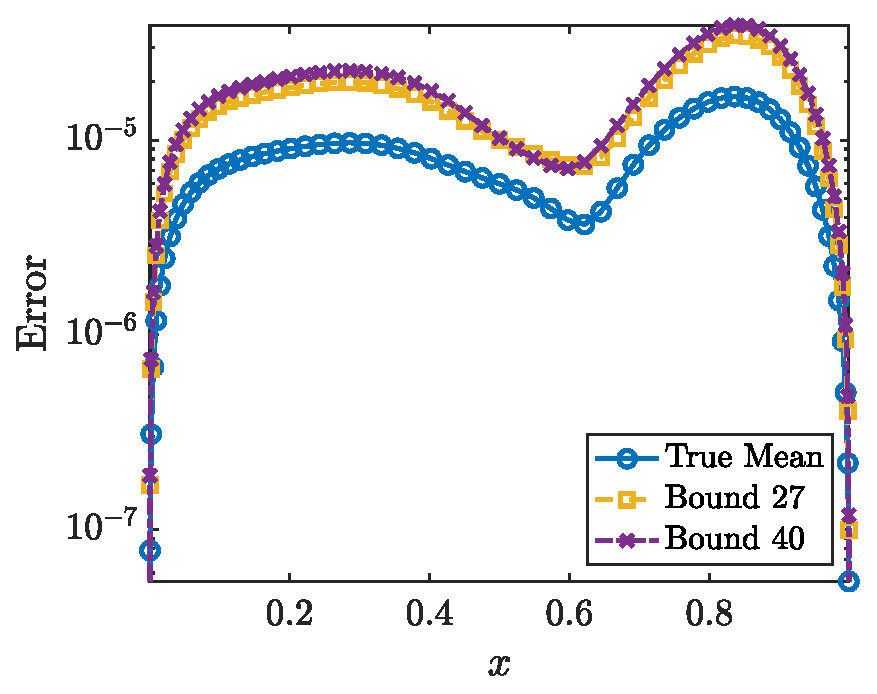
\includegraphics[width =0.6\textwidth]{Figures/LDC_eq_27_bound.eps}
\caption{LDC Comparison of the true mean error and the bound calculated from equation (\ref{eq:bound_presum}) for all $M$ points. The mean error for each point is computed from $N=200$ samples and the square root has been taken.} 
\label{fig:LDC_eq_27_bound}
\end{figure}
%
% 
\begin{figure}[ht!]
\centering
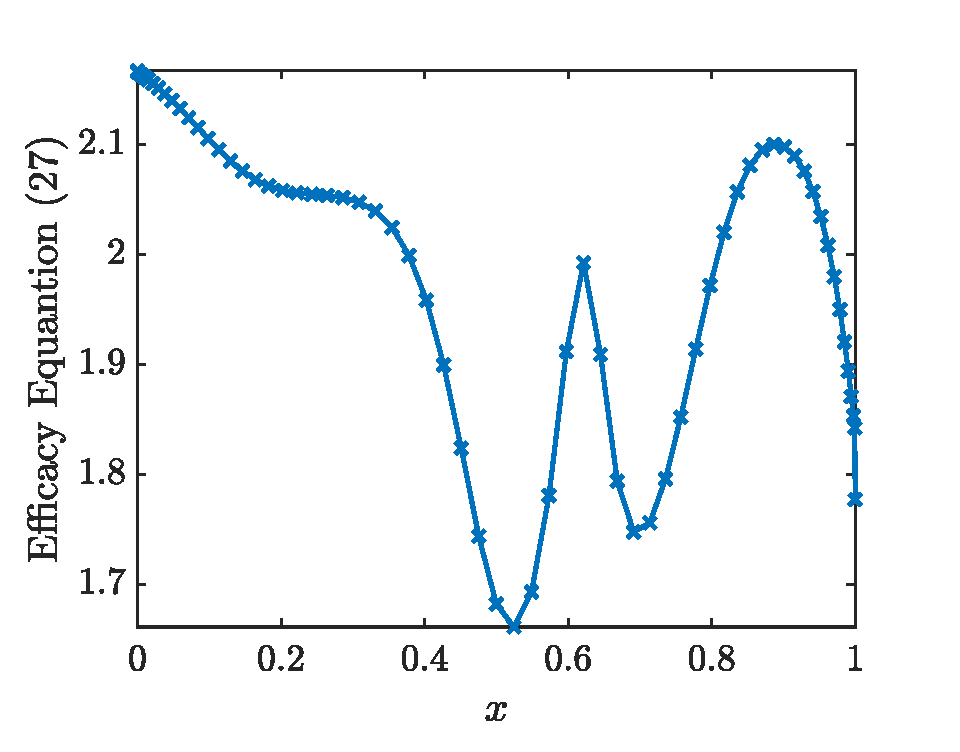
\includegraphics[width =0.6\textwidth]{Figures/LDC_eq_27_efficacy.eps}
\caption{LDC Error bound efficacy in equation (\ref{eq:bound_presum}) for all $M$ points. The mean error for each point is computed from $N=200$ samples and the square root has been taken.} 
\label{fig:LDC_eq_27_efficacy}
\end{figure}
%

Next we plot $\Theta_{N_H}$ as a function of $x$ in Figure \ref{fig:LDC_theta}. We find that $\Theta$ exhibits entirely reasonable values, ie close to 1, and the maximum value is no cause for concern. 
% 
\begin{figure}[ht!]
\centering
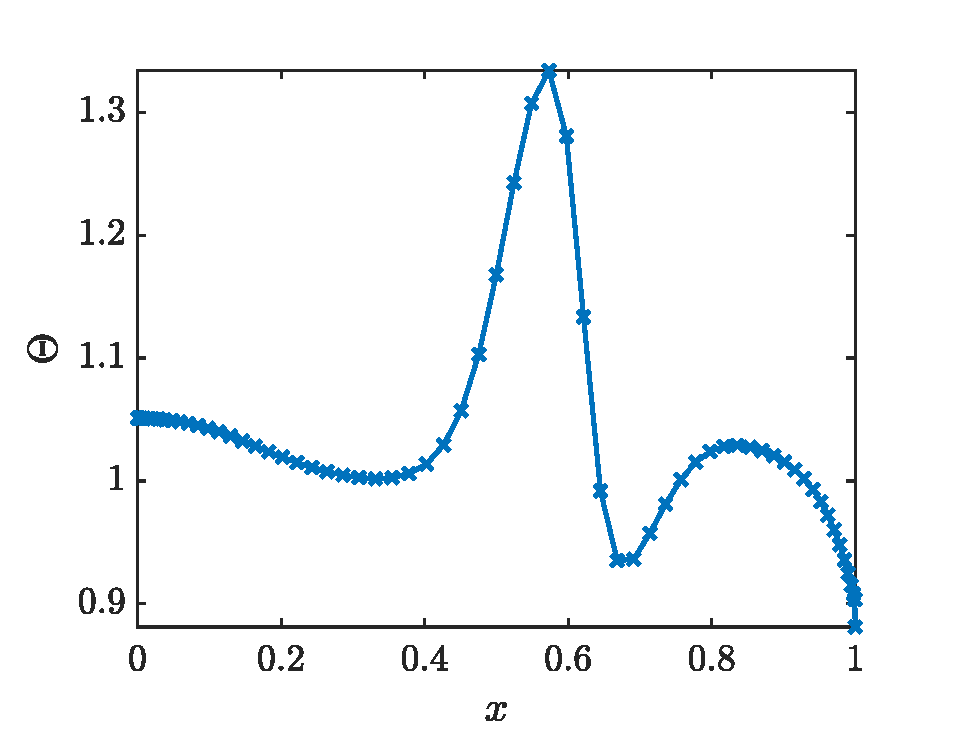
\includegraphics[width =0.6\textwidth]{Figures/LDC_theta.eps}
\caption{LDC $\Theta_{N_h}$ as a function of location in $x$.} 
\label{fig:LDC_theta}
\end{figure}
%

Finally, we plot $Y_{N_H}$ as a function of $x$ in Figure \ref{fig:LDC_Y}. It is immediately apparent that several very large peaks occur in $Y$, while most of the values are much more reasonable. To examine this we plot the two terms that comprise $Y_{N_H}$ from equation (\ref{eq:Y}) in Figure \ref{fig:LDC_Y_ratio}. We find that the error of the matrix ID estimate in Figure \ref{fig:LDC_Y_ratio} tends to be smaller than the error of the PC bi-fidelity estimate. It is clear that where the matrix ID error is close to $0$ $Y_{N_H}$ becomes very large and in turn causes the bound summed over all points that uses the maximum of $Y$ to perform poorly in efficacy.  \\
% 
\begin{figure}[ht!]
\centering
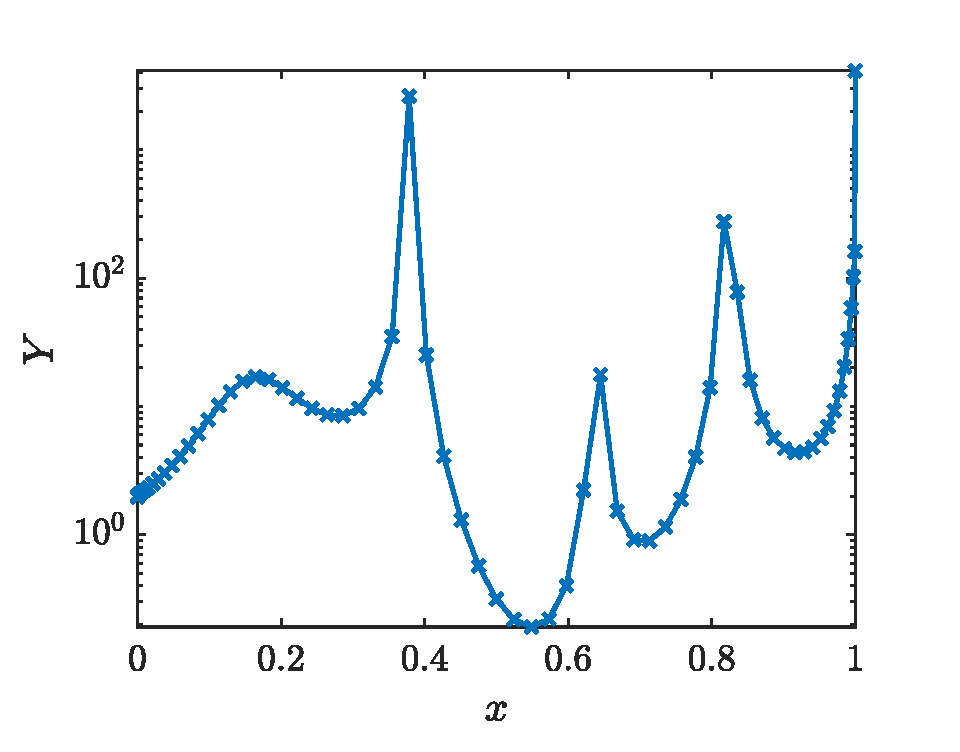
\includegraphics[width =0.6\textwidth]{Figures/LDC_Y.eps}
\caption{LDC $Y_{N_h}$ as a function of location in $x$.} 
\label{fig:LDC_Y}
\end{figure}
%
% 
\begin{figure}[ht!]
\centering
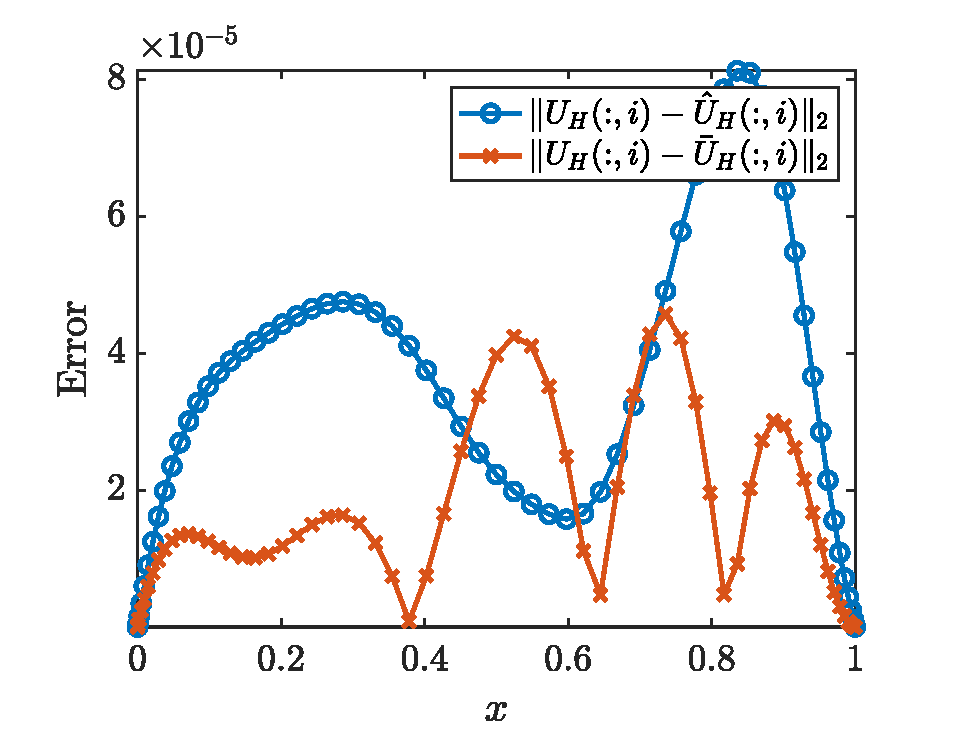
\includegraphics[width =0.6\textwidth]{Figures/LDC_Y_ratio.eps}
\caption{LDC Terms that comprise $Y_{N_h}$ as a function of location in $x$.} 
\label{fig:LDC_Y_ratio}
\end{figure}
%


Numerical Test Case II: Gas Turbine: \\

For full details of the Gas Turbine model please refer to the paper draft. The problem can be thought of as heated flow past a cylidner. In this test case we consider two separate QoI, the temperature along a vertical line at $x=0.2$ and temperature around the entire cylinder surface from $-\pi$ to $\pi$ radians. The vertical line has $M=128$ points while the cylinder surface has $M=202$. Both sets of coordinates are represented by $x$ in this study. 
For both QoI we estimate $N=100$ samples with $N_H = 20$ high-fidelity samples, a bi-fidelity rank of $r=8$, $R=18$ samples to compute the matrix ID error bound $\rho_k(\tau)$ and $N_{H_\infty}=200$. 

Gas turbine temperature along vertical line figure summary: 
\begin{itemize}
\item Figure \ref{fig:GT_mid_eq_27_bound} plots mean error for each point alongside the corresponding point specific bound from equation (\ref{eq:bound_presum}) 
\item Figure \ref{fig:GT_mid_eq_27_efficacy} shows efficacy of equation (\ref{eq:bound_presum}) for each point
\item Figure \ref{fig:GT_mid_theta} plots $\Theta_{N_H}$ as a function of $x$
\item Figure \ref{fig:GT_mid_Y} plots $Y_{N_H}$ as a function of $x$
\item Figure \ref{fig:GT_mid_Y_ratio} plots the two terms that comprise $Y_{N_H}$ from equation (\ref{eq:Y})
\end{itemize}

Gas turbine temperature around cylinder surface figure summary: 
\begin{itemize}
\item Figure \ref{fig:GT_cylinder_eq_27_bound} plots mean error for each point alongside the corresponding point specific bound from equation (\ref{eq:bound_presum}) 
\item Figure \ref{fig:GT_cylinder_eq_27_efficacy} shows efficacy of equation (\ref{eq:bound_presum}) for each point
\item Figure \ref{fig:GT_cylinder_theta} plots $\Theta_{N_H}$ as a function of $x$
\item Figure \ref{fig:GT_cylinder_Y} plots $Y_{N_H}$ as a function of $x$
\item Figure \ref{fig:GT_cylinder_Y_ratio} plots the two terms that comprise $Y_{N_H}$ from equation (\ref{eq:Y})
\end{itemize}

% 
\begin{figure}[ht!]
\centering
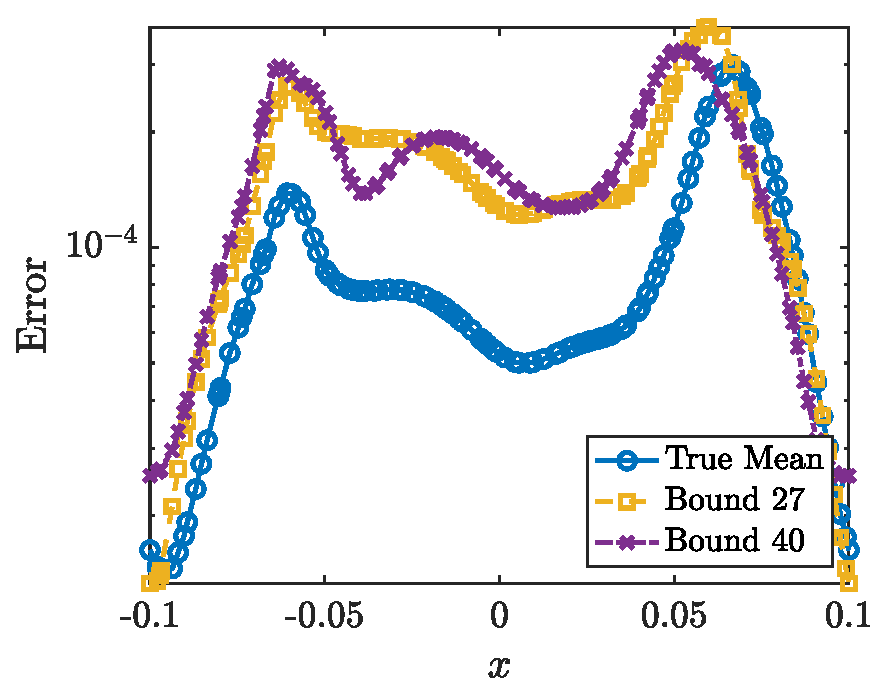
\includegraphics[width =0.6\textwidth]{Figures/GT_mid_eq_27_bound.eps}
\caption{Gas turbine vertical line. Comparison of the true mean error and the bound calculated from equation (\ref{eq:bound_presum}) for all $M$ points. The mean error for each point is computed from $N=200$ samples and the square root has been taken.} 
\label{fig:GT_mid_eq_27_bound}
\end{figure}
%

\begin{figure}[ht!]
\centering
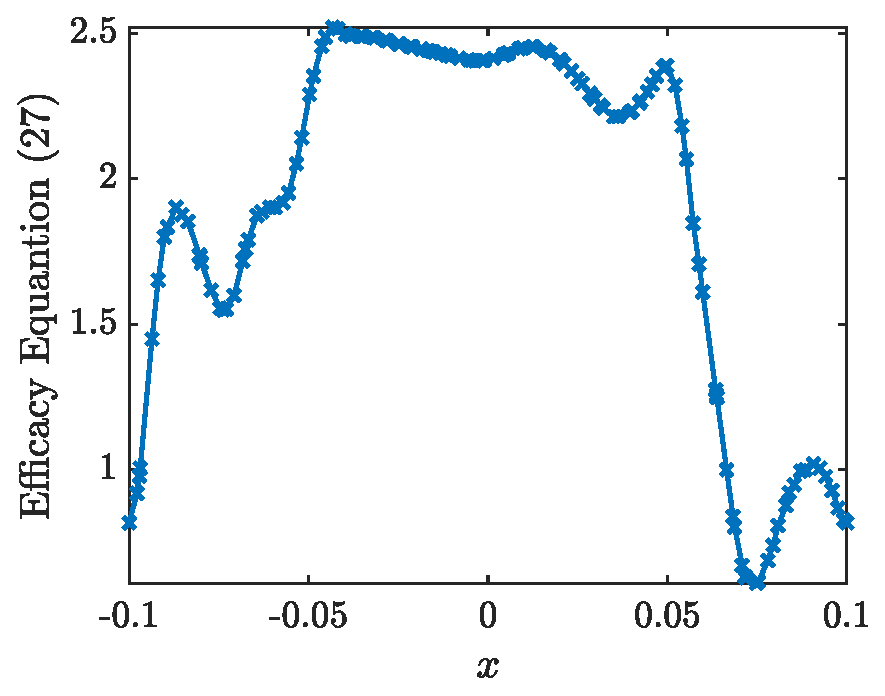
\includegraphics[width =0.6\textwidth]{Figures/GT_mid_eq_27_efficacy.eps}
\caption{Gas turbine vertical line. Error bound efficacy in equation (\ref{eq:bound_presum}) for all $M$ points. The mean error for each point is computed from $N=200$ samples and the square root has been taken.} 
\label{fig:GT_mid_eq_27_efficacy}
\end{figure}
%

% 
\begin{figure}[ht!]
\centering
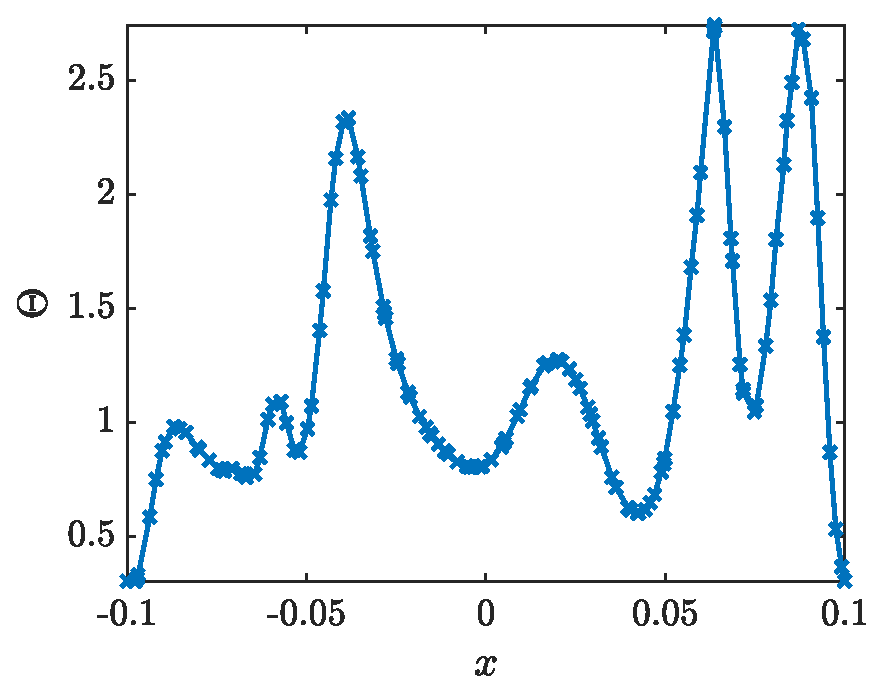
\includegraphics[width =0.6\textwidth]{Figures/GT_mid_theta.eps}
\caption{Gas turbine vertical line. $\Theta_{N_h}$ as a function of location in $x$.} 
\label{fig:GT_mid_theta}
\end{figure}
%

% 
\begin{figure}[ht!]
\centering
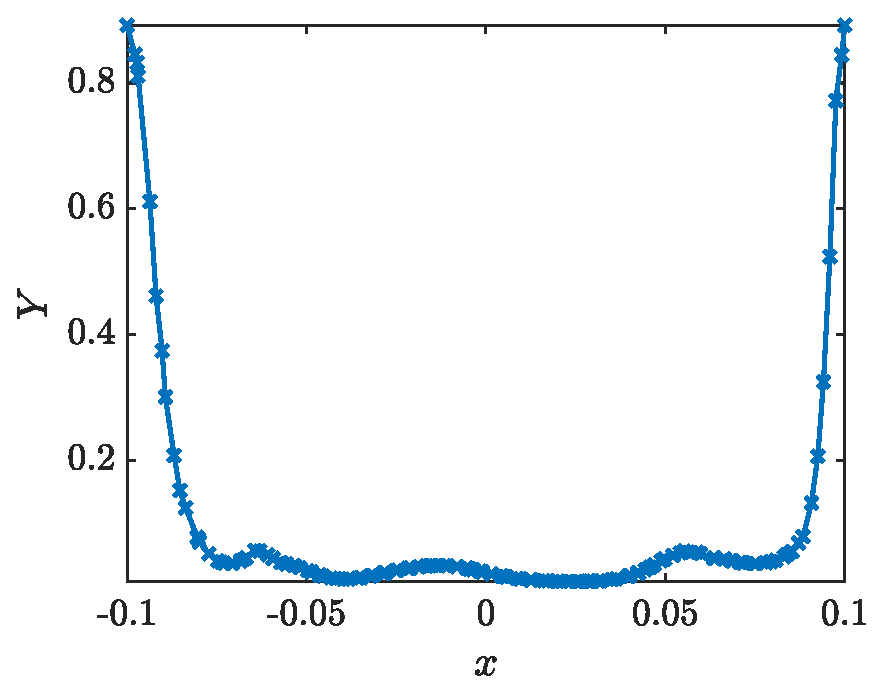
\includegraphics[width =0.6\textwidth]{Figures/GT_mid_Y.eps}
\caption{Gas turbine vertical line. $Y_{N_h}$ as a function of location in $x$.} 
\label{fig:GT_mid_Y}
\end{figure}
%
% 
\begin{figure}[ht!]
\centering
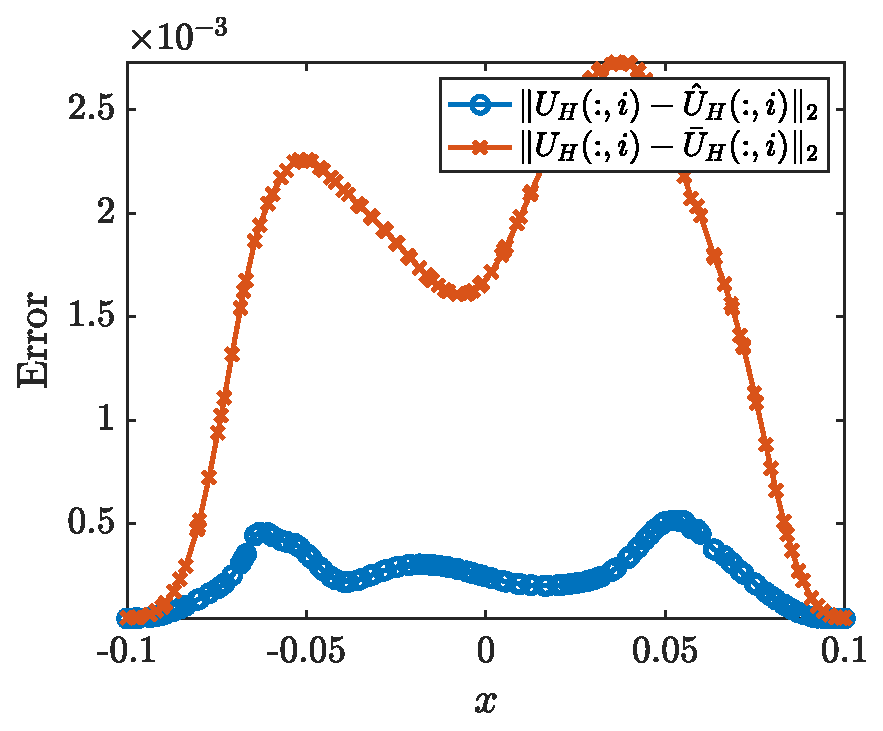
\includegraphics[width =0.6\textwidth]{Figures/GT_mid_Y_ratio.eps}
\caption{Gas turbine vertical line. Terms that comprise $Y_{N_h}$ as a function of location in $x$.} 
\label{fig:GT_mid_Y_ratio}
\end{figure}
%

%%% cylinder

% 
\begin{figure}[ht!]
\centering
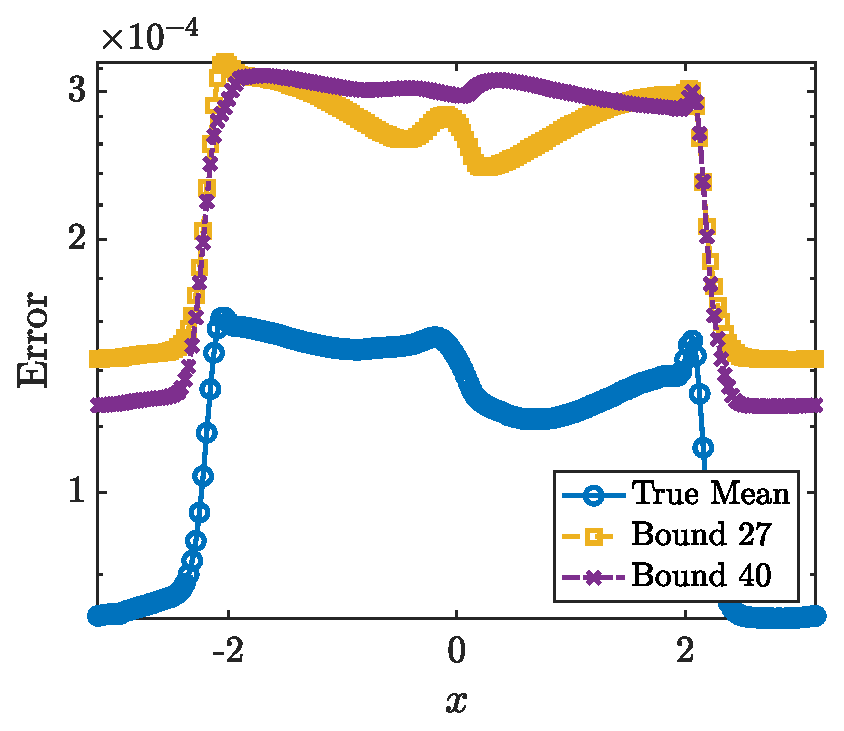
\includegraphics[width =0.6\textwidth]{Figures/GT_cylinder_eq_27_bound.eps}
\caption{Gas turbine cylinder. Comparison of the true mean error and the bound calculated from equation (\ref{eq:bound_presum}) for all $M$ points. The mean error for each point is computed from $N=200$ samples and the square root has been taken.} 
\label{fig:GT_cylinder_eq_27_bound}
\end{figure}
%

\begin{figure}[ht!]
\centering
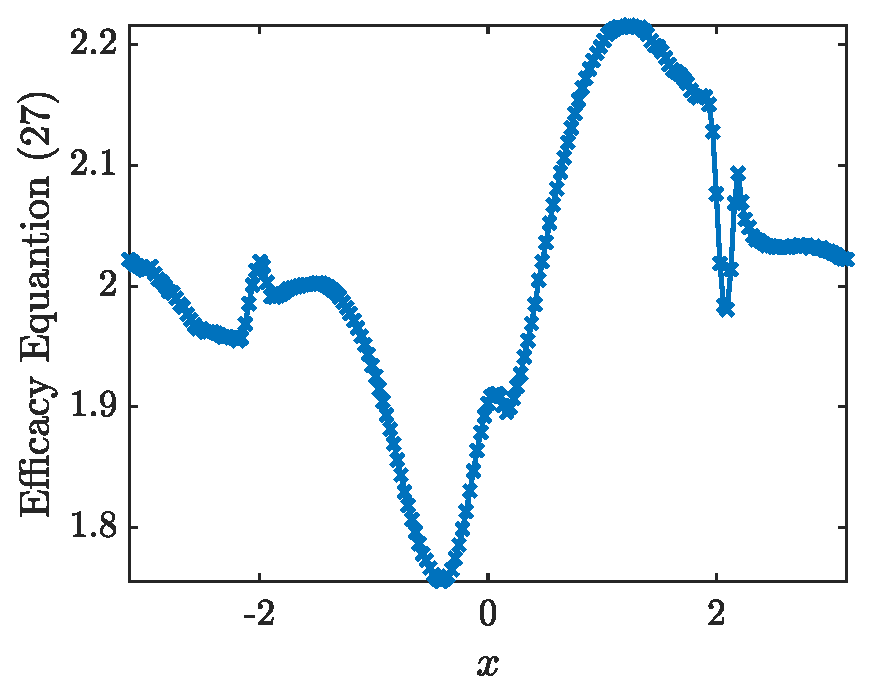
\includegraphics[width =0.6\textwidth]{Figures/GT_cylinder_eq_27_efficacy.eps}
\caption{Gas turbine cylinder. Error bound efficacy in equation (\ref{eq:bound_presum}) for all $M$ points. The mean error for each point is computed from $N=200$ samples and the square root has been taken.} 
\label{fig:GT_cylinder_eq_27_efficacy}
\end{figure}
%

% 
\begin{figure}[ht!]
\centering
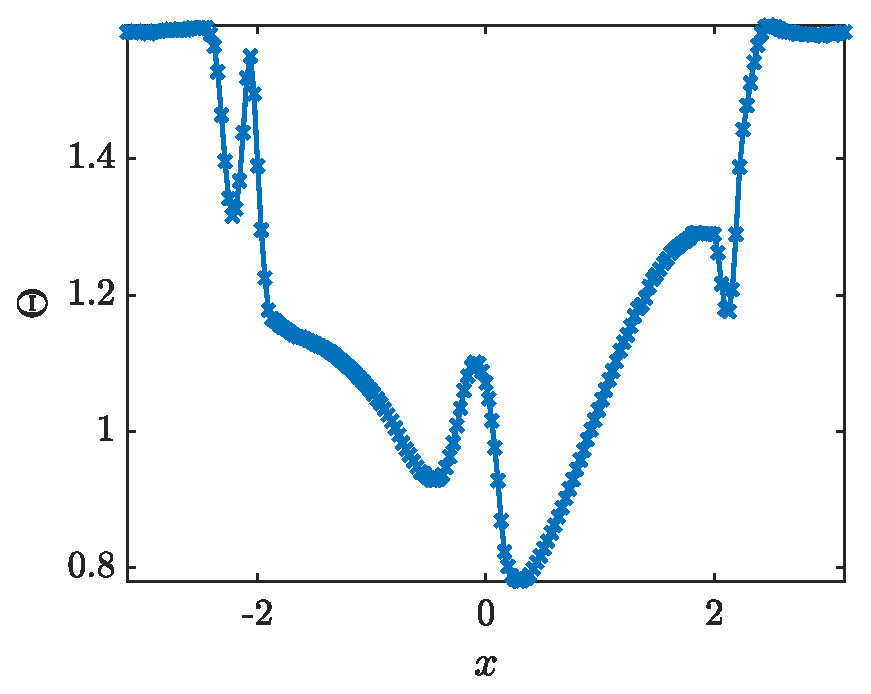
\includegraphics[width =0.6\textwidth]{Figures/GT_cylinder_theta.eps}
\caption{Gas turbine cylinder. $\Theta_{N_h}$ as a function of location in $x$.} 
\label{fig:GT_cylinder_theta}
\end{figure}
%

% 
\begin{figure}[ht!]
\centering
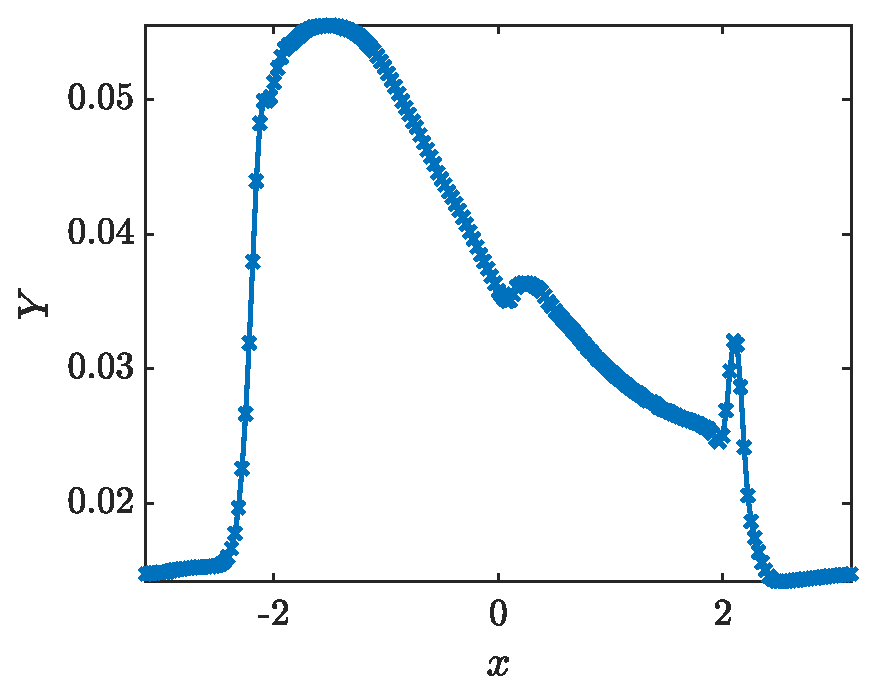
\includegraphics[width =0.6\textwidth]{Figures/GT_cylinder_Y.eps}
\caption{Gas turbine cylinder. $Y_{N_h}$ as a function of location in $x$.} 
\label{fig:GT_cylinder_Y}
\end{figure}
%
% 
\begin{figure}[ht!]
\centering
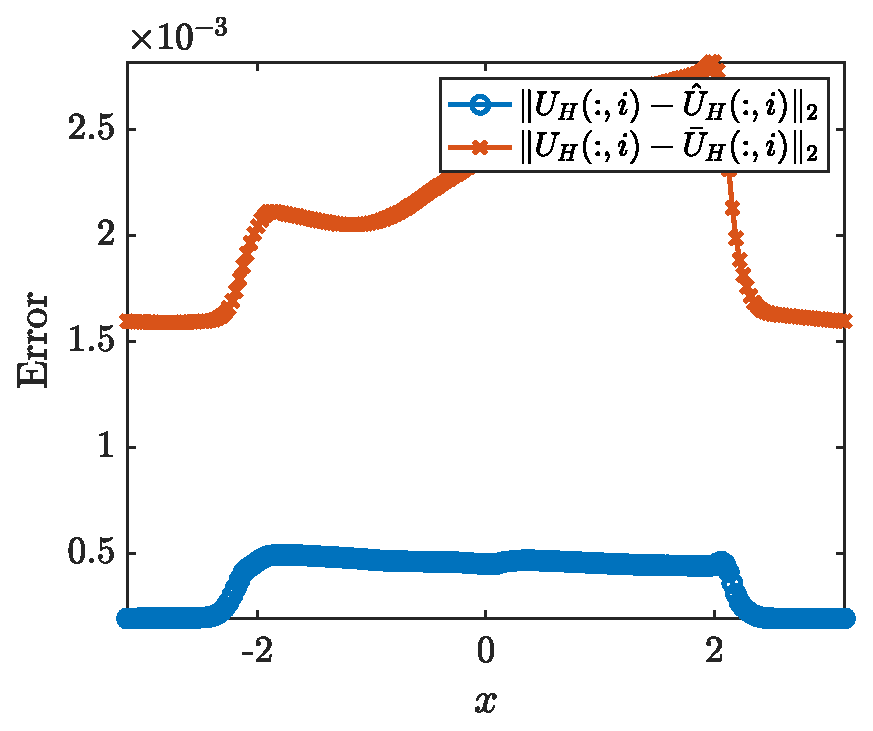
\includegraphics[width =0.6\textwidth]{Figures/GT_cylinder_Y_ratio.eps}
\caption{Gas turbine cylinder. Terms that comprise $Y_{N_h}$ as a function of location in $x$.} 
\label{fig:GT_cylinder_Y_ratio}
\end{figure}
%


Numerical Test Case III: Airfoil: \\

For full details of the Airfoil model please refer to the paper draft. In this test case the QoI is the coefficient of pressure at $M=200$ points evenly spaced around the airfoil's surface, mapped to $x$ $-1$ to $1$. We estimate $N=200$ samples with $N_H = 20$ high-fidelity samples, a bi-fidelity rank of $r=5$, $R=15$ samples to compute the matrix ID error bound $\rho_k(\tau)$ and $N_{H_\infty}=500$. 

Airfoil figure summary: 
\begin{itemize}
\item Figure \ref{fig:Airfoil_eq_27_bound} plots mean error for each point alongside the corresponding point specific bound from equation (\ref{eq:bound_presum}) 
\item Figure \ref{fig:Airfoil_eq_27_efficacy} shows efficacy of equation (\ref{eq:bound_presum}) for each point
\item Figure \ref{fig:Airfoil_theta} plots $\Theta_{N_H}$ as a function of $x$
\item Figure \ref{fig:Airfoil_Y} plots $Y_{N_H}$ as a function of $x$
\item Figure \ref{fig:Airfoil_Y_ratio} plots the two terms that comprise $Y_{N_H}$ from equation (\ref{eq:Y})
\end{itemize}

% 
\begin{figure}[ht!]
\centering
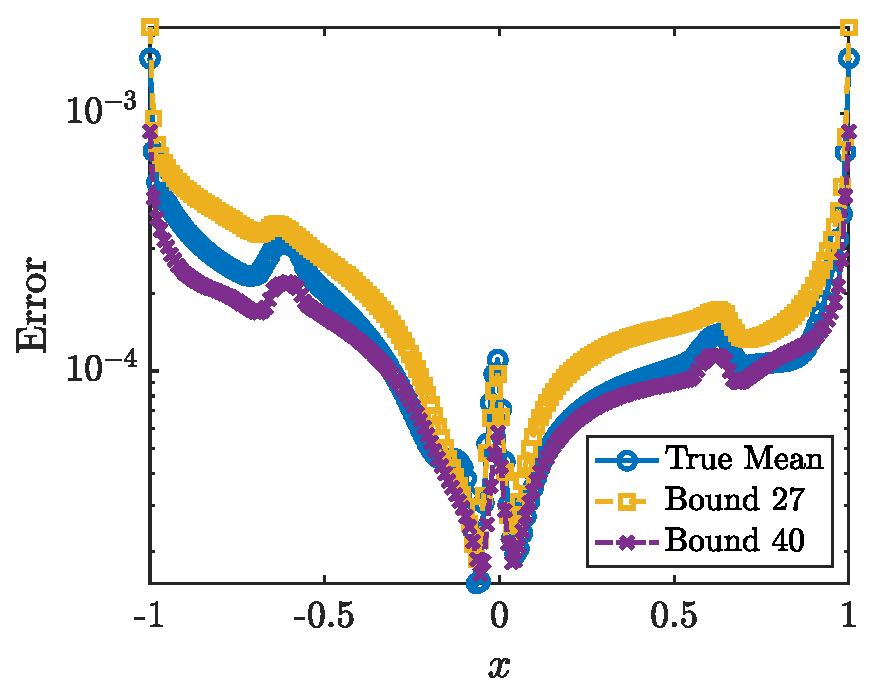
\includegraphics[width =0.6\textwidth]{Figures/Airfoil_eq_27_bound.eps}
\caption{Airfoil Comparison of the true mean error and the bound calculated from equation (\ref{eq:bound_presum}) for all $M$ points. The mean error for each point is computed from $N=200$ samples and the square root has been taken.} 
\label{fig:Airfoil_eq_27_bound}
\end{figure}
%

\begin{figure}[ht!]
\centering
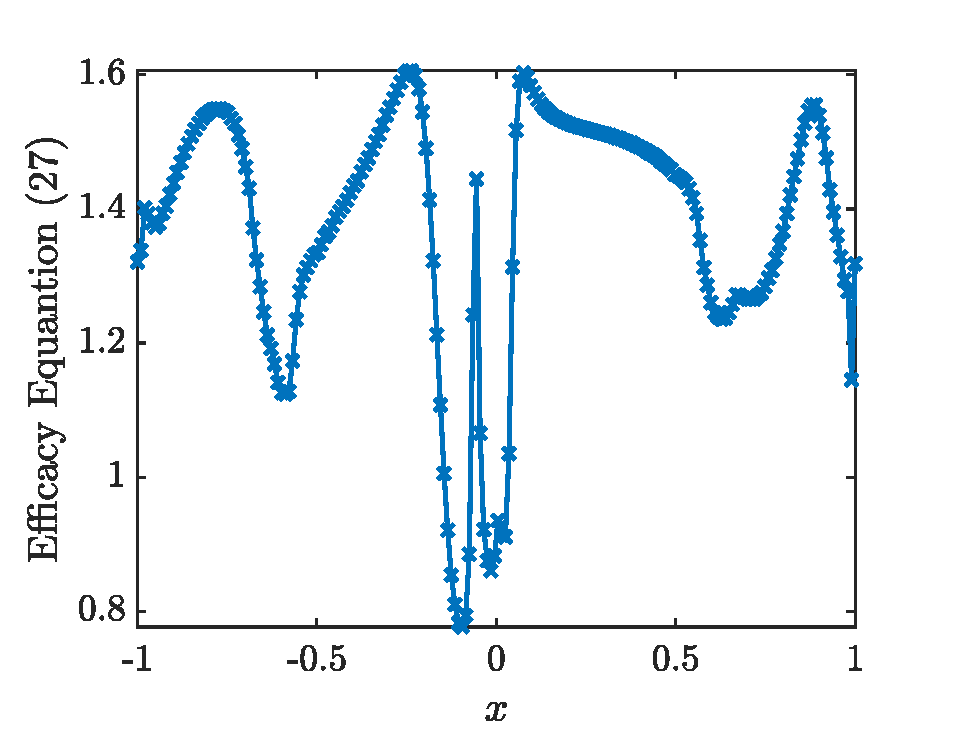
\includegraphics[width =0.6\textwidth]{Figures/Airfoil_eq_27_efficacy.eps}
\caption{Airfoil Error bound efficacy in equation (\ref{eq:bound_presum}) for all $M$ points. The mean error for each point is computed from $N=200$ samples and the square root has been taken.} 
\label{fig:Airfoil_eq_27_efficacy}
\end{figure}
%

% 
\begin{figure}[ht!]
\centering
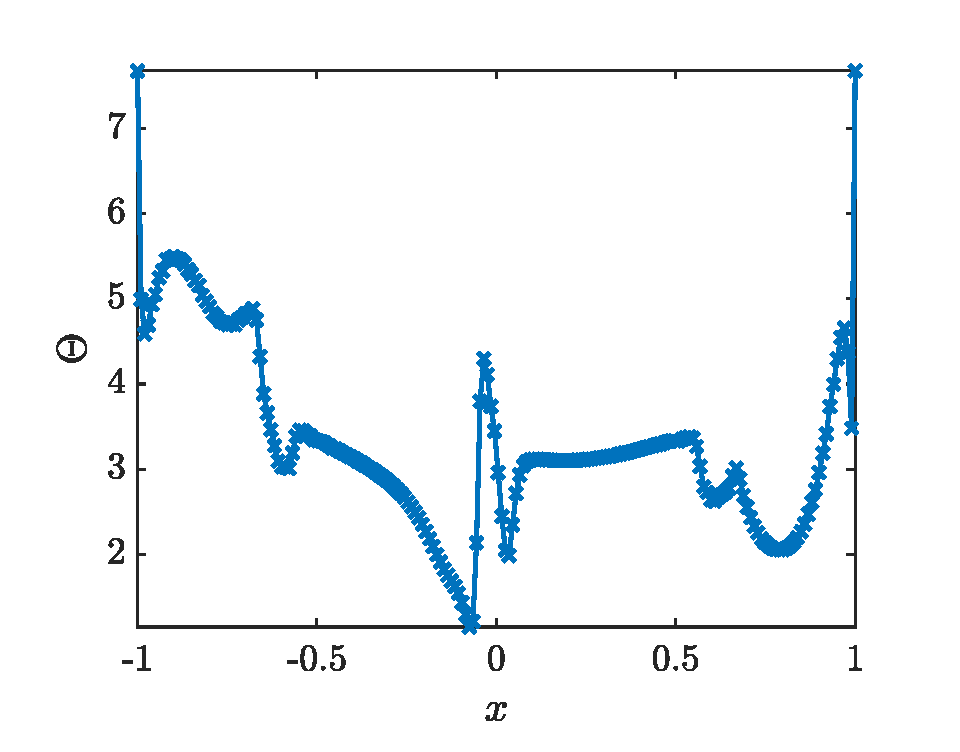
\includegraphics[width =0.6\textwidth]{Figures/Airfoil_theta.eps}
\caption{Airfoil $\Theta_{N_h}$ as a function of location in $x$.} 
\label{fig:Airfoil_theta}
\end{figure}
%

% 
\begin{figure}[ht!]
\centering
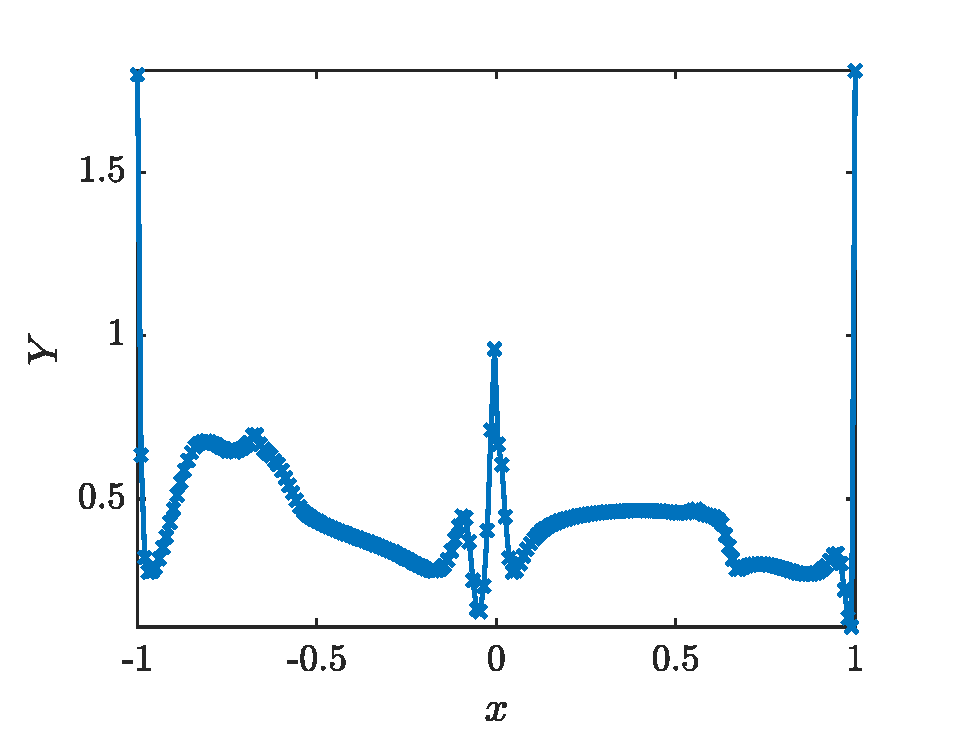
\includegraphics[width =0.6\textwidth]{Figures/Airfoil_Y.eps}
\caption{Airfoil $Y_{N_h}$ as a function of location in $x$.} 
\label{fig:Airfoil_Y}
\end{figure}
%
% 
\begin{figure}[ht!]
\centering
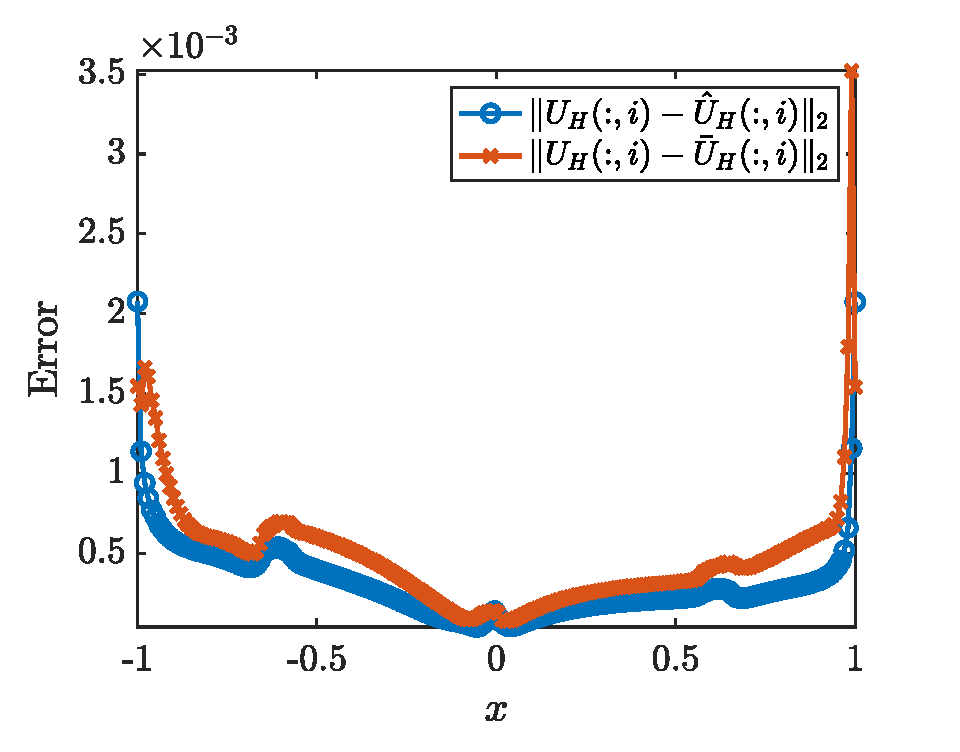
\includegraphics[width =0.6\textwidth]{Figures/Airfoil_Y_ratio.eps}
\caption{Airfoil Terms that comprise $Y_{N_h}$ as a function of location in $x$.} 
\label{fig:Airfoil_Y_ratio}
\end{figure}
%


% 
\begin{figure}[ht!]
\centering
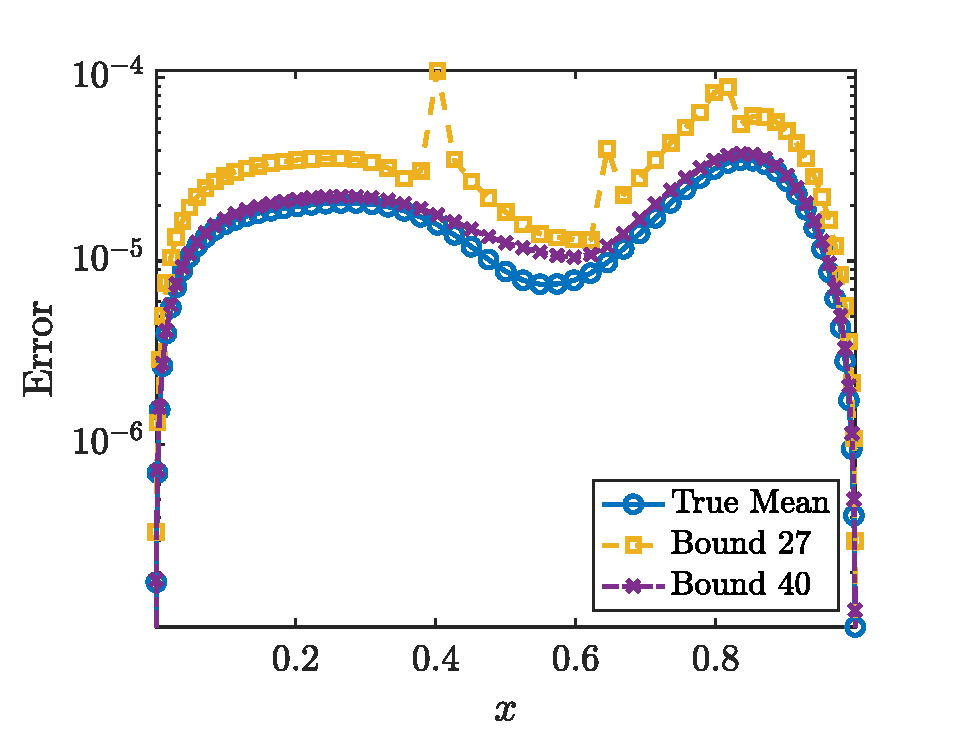
\includegraphics[width =0.6\textwidth]{Figures/LDC_eq_27_bound_30reps.eps}
\caption{LDC Comparison of the true mean error and the bound calculated from equations (\ref{eq:bound_presum}) and (\ref{eq:bound_vector}) for all $M$ points. The mean error for each point is computed from $N=200$ samples and the square root has been taken. The error bound is computed from the average of $30$ repetitions.} 
\label{fig:LDC_eq_27_bound_reps}
\end{figure}
%

% 
\begin{figure}[ht!]
\centering
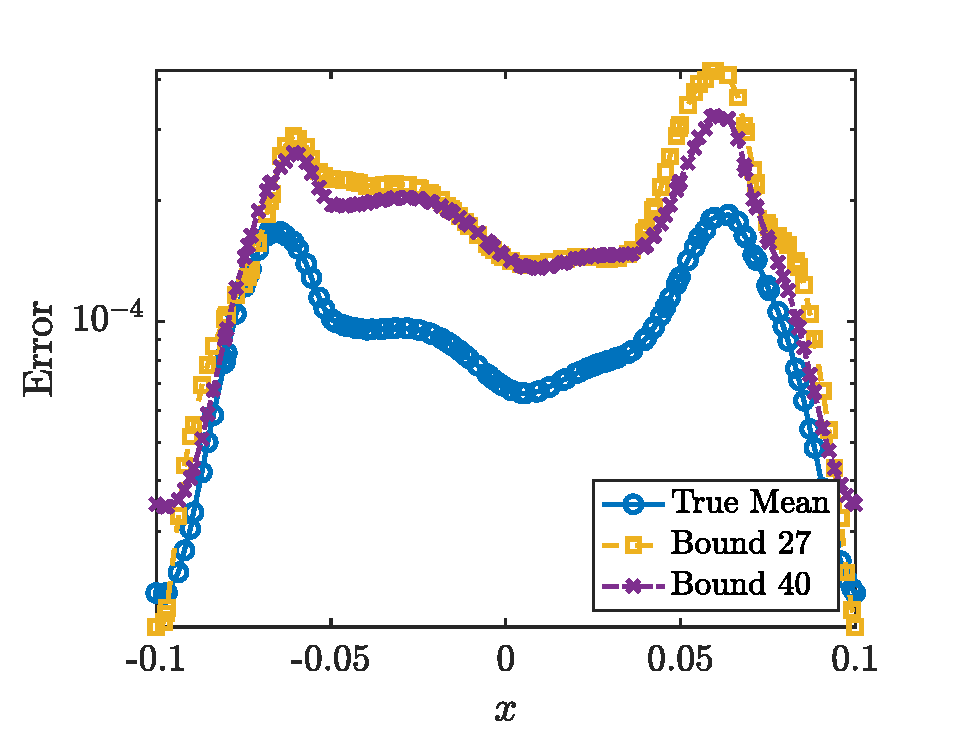
\includegraphics[width =0.6\textwidth]{Figures/GT_mid_eq_27_bound_30reps.eps}
\caption{Gas turbine vertical line. Comparison of the true mean error and the bound calculated from equation (\ref{eq:bound_presum}) for all $M$ points. The mean error for each point is computed from $N=200$ samples and the square root has been taken.} 
\label{fig:GT_mid_eq_27_bound_reps}
\end{figure}
%

% 
\begin{figure}[ht!]
\centering
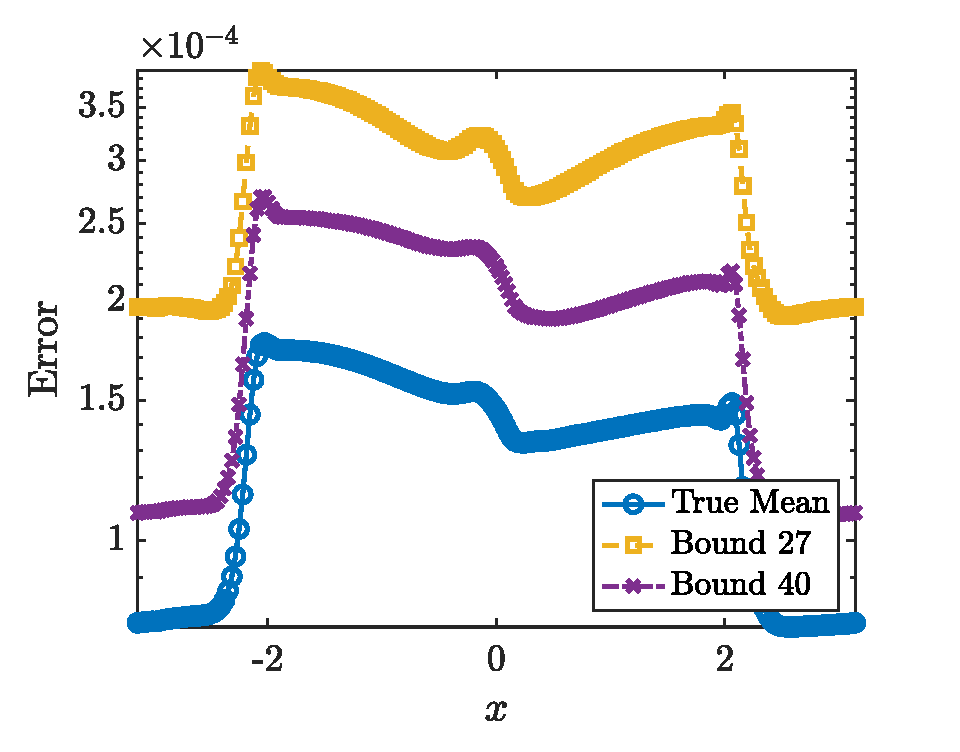
\includegraphics[width =0.6\textwidth]{Figures/GT_cylinder_eq_27_bound_30reps.eps}
\caption{Gas turbine cylinder. Comparison of the true mean error and the bound calculated from equation (\ref{eq:bound_presum}) for all $M$ points. The mean error for each point is computed from $N=200$ samples and the square root has been taken. The error bound is computed from the average of $30$ repetitions.} 
\label{fig:GT_cylinder_eq_27_bound_reps}
\end{figure}
%



% 
\begin{figure}[ht!]
\centering
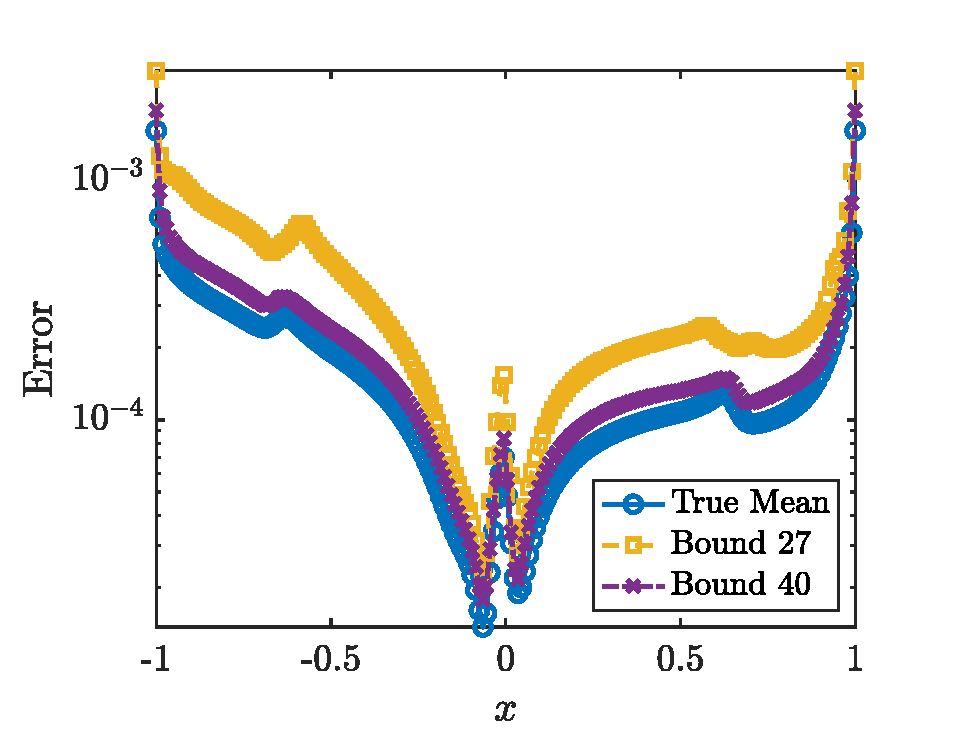
\includegraphics[width =0.6\textwidth]{Figures/Airfoil_eq_27_bound_30reps.eps}
\caption{Airfoil Comparison of the true mean error and the bound calculated from equations (\ref{eq:bound_presum}) and (\ref{eq:bound_vector}) for all $M$ points. The mean error for each point is computed from $N=200$ samples and the square root has been taken. The error bound is computed from the average of 30 repetitions.} 
\label{fig:Airfoil_eq_27_bound_reps}
\end{figure}
%

\end{document}
